% !TEX root = JKPS_TeX_sample_eps.tex

\section{Study with \pythia}
\label{sec:ana}
The string shoving model is quantitatively studied by analyzing charged hadrons from millions of non-diffractive \pythia \pp events at $\sqrt{s}=13~\mathrm{TeV}$. 
The event multiplicity is defined with charged hadrons satisfying $|\eta|<$~2.4 and $\pt>$~0.4~GeV/$c$, which is equivalent definition to the experimental results.
To calculate two-particle correlations, we follow the formula for per-trigger yields~\cite{Khachatryan:2015lva}, which is defined as, 
\begin{align}
    \frac{1}{N_{\rm{trig}}} \frac{ {\rm d^{2}} N_{\rm{pair}} }{ \rm{d}\deta \rm{d}\dphi} = B(0,0)\frac{S(\deta, \dphi)}{B(\deta, \dphi)},
\end{align}
where $N_\mathrm{trig}$ and $N_\mathrm{pair}$ are the number of trigger particles and the number of pairs, respectively.
$S (\Delta\eta, \Delta\varphi)$ and $B(\Delta\eta, \Delta\varphi)$ are per-trigger yields in same and mixed events:
\begin{align}
    S(\deta,\dphi) &= \frac{1}{N_{{\rm trig}}} \frac{ {\rm d^{2}} N_{\rm{pair}}^{\rm same} }{ \rm{d}\deta \rm{d}\dphi},\\
    B(\deta,\dphi) &= \frac{1}{N_{{\rm trig}}} \frac{ {\rm d^{2}} N_{\rm{pair}}^{\rm mixed} }{ \rm{d}\deta \rm{d}\dphi},
\end{align}
and $B(0, 0)$ is the per-trigger yield at $(\deta,\dphi)=(0,0)$, where the pair acceptance is maximum.

\begin{figure}[tbh]
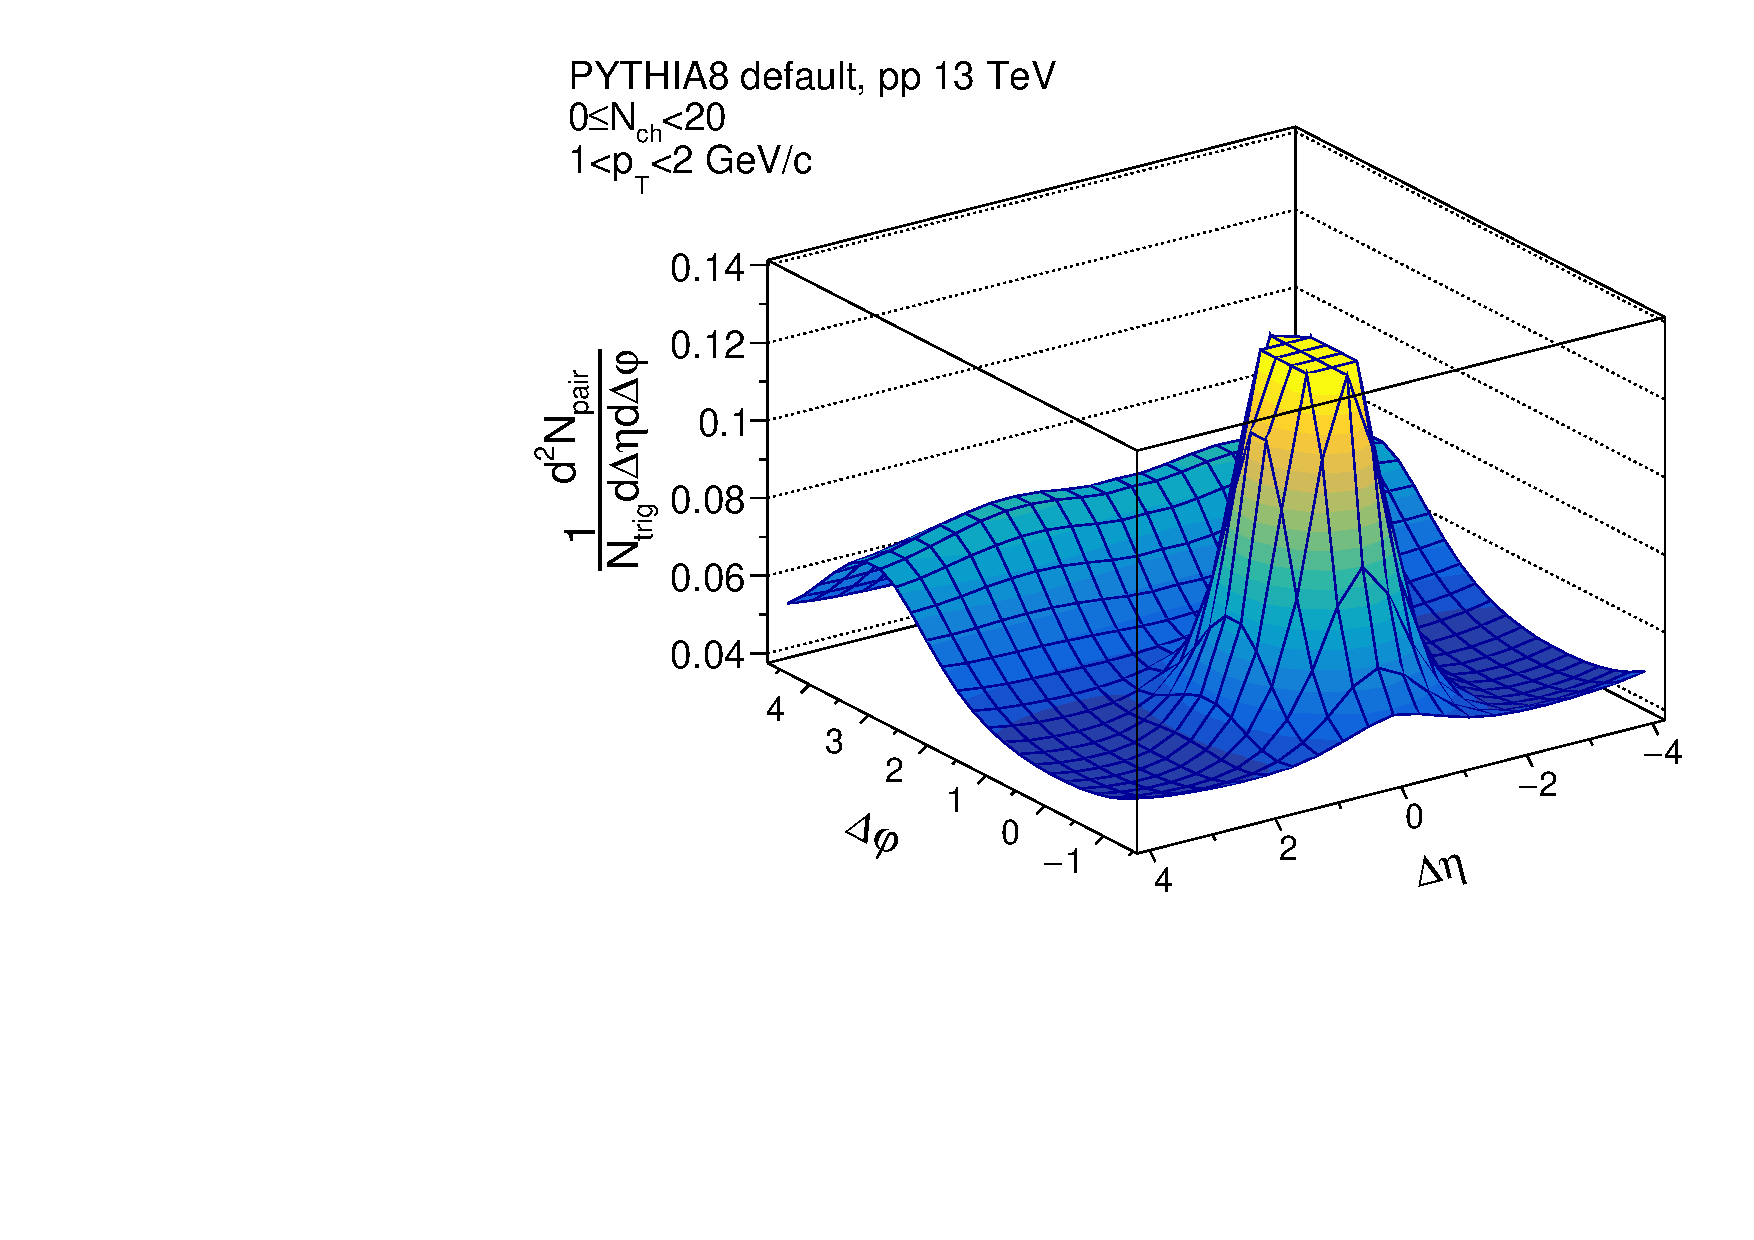
\includegraphics[width=0.49\textwidth]{figures/2D_default_lo_final.pdf}
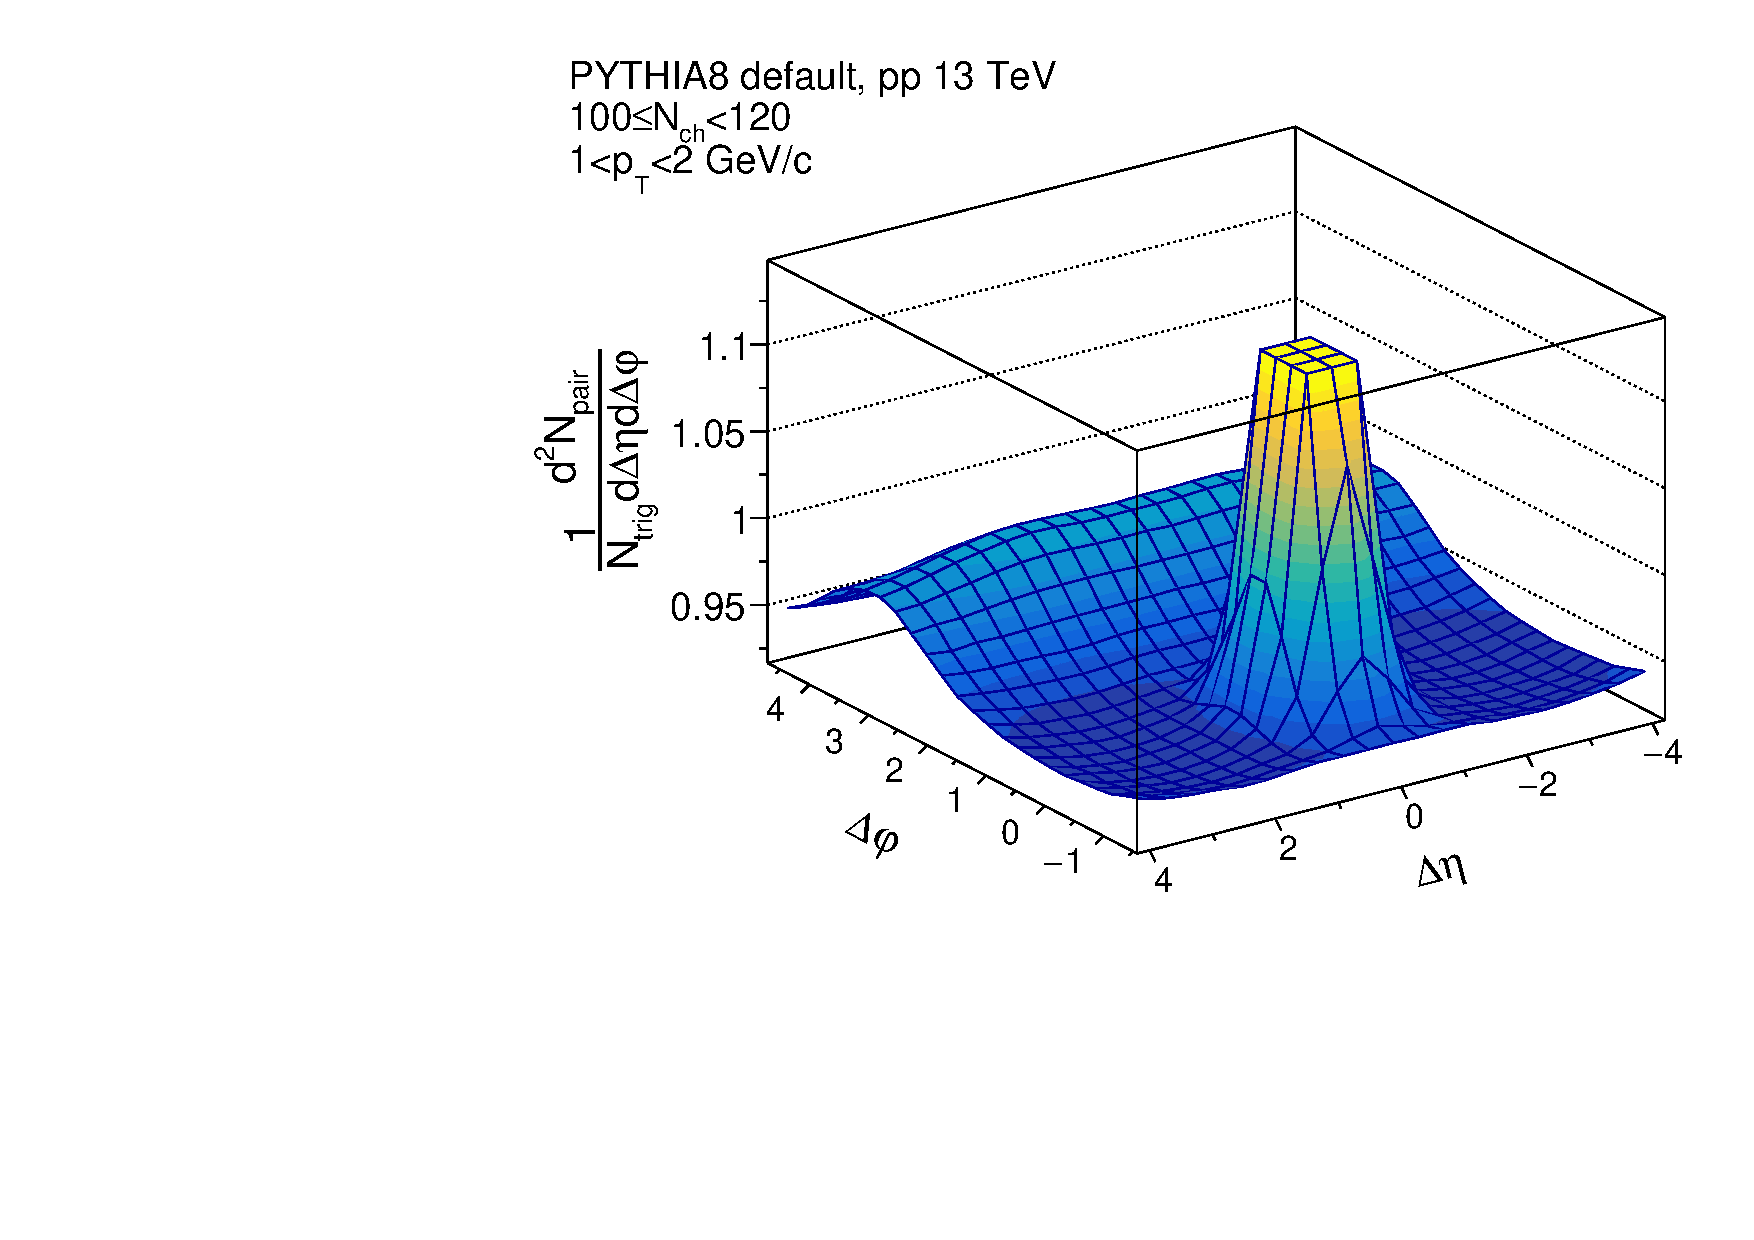
\includegraphics[width=0.49\textwidth]{figures/2D_default_hi_final.pdf}
\caption{Two-particle correlation functions for charged hadrons in $|\eta|<$~2.4 and 1~$<\pt<$~2~GeV/$c$ from low (left) and high (right) multiplicity \pythia \pp events at $\sqrt{s}=$~13~TeV with the default configuration. \Nch is calculated with charged hadrons in $|\eta|<$~2.4 and $\pt>$~0.4~GeV/$c$.}
\label{fig:2d_default_final}
\end{figure}

\begin{figure}[tbh]
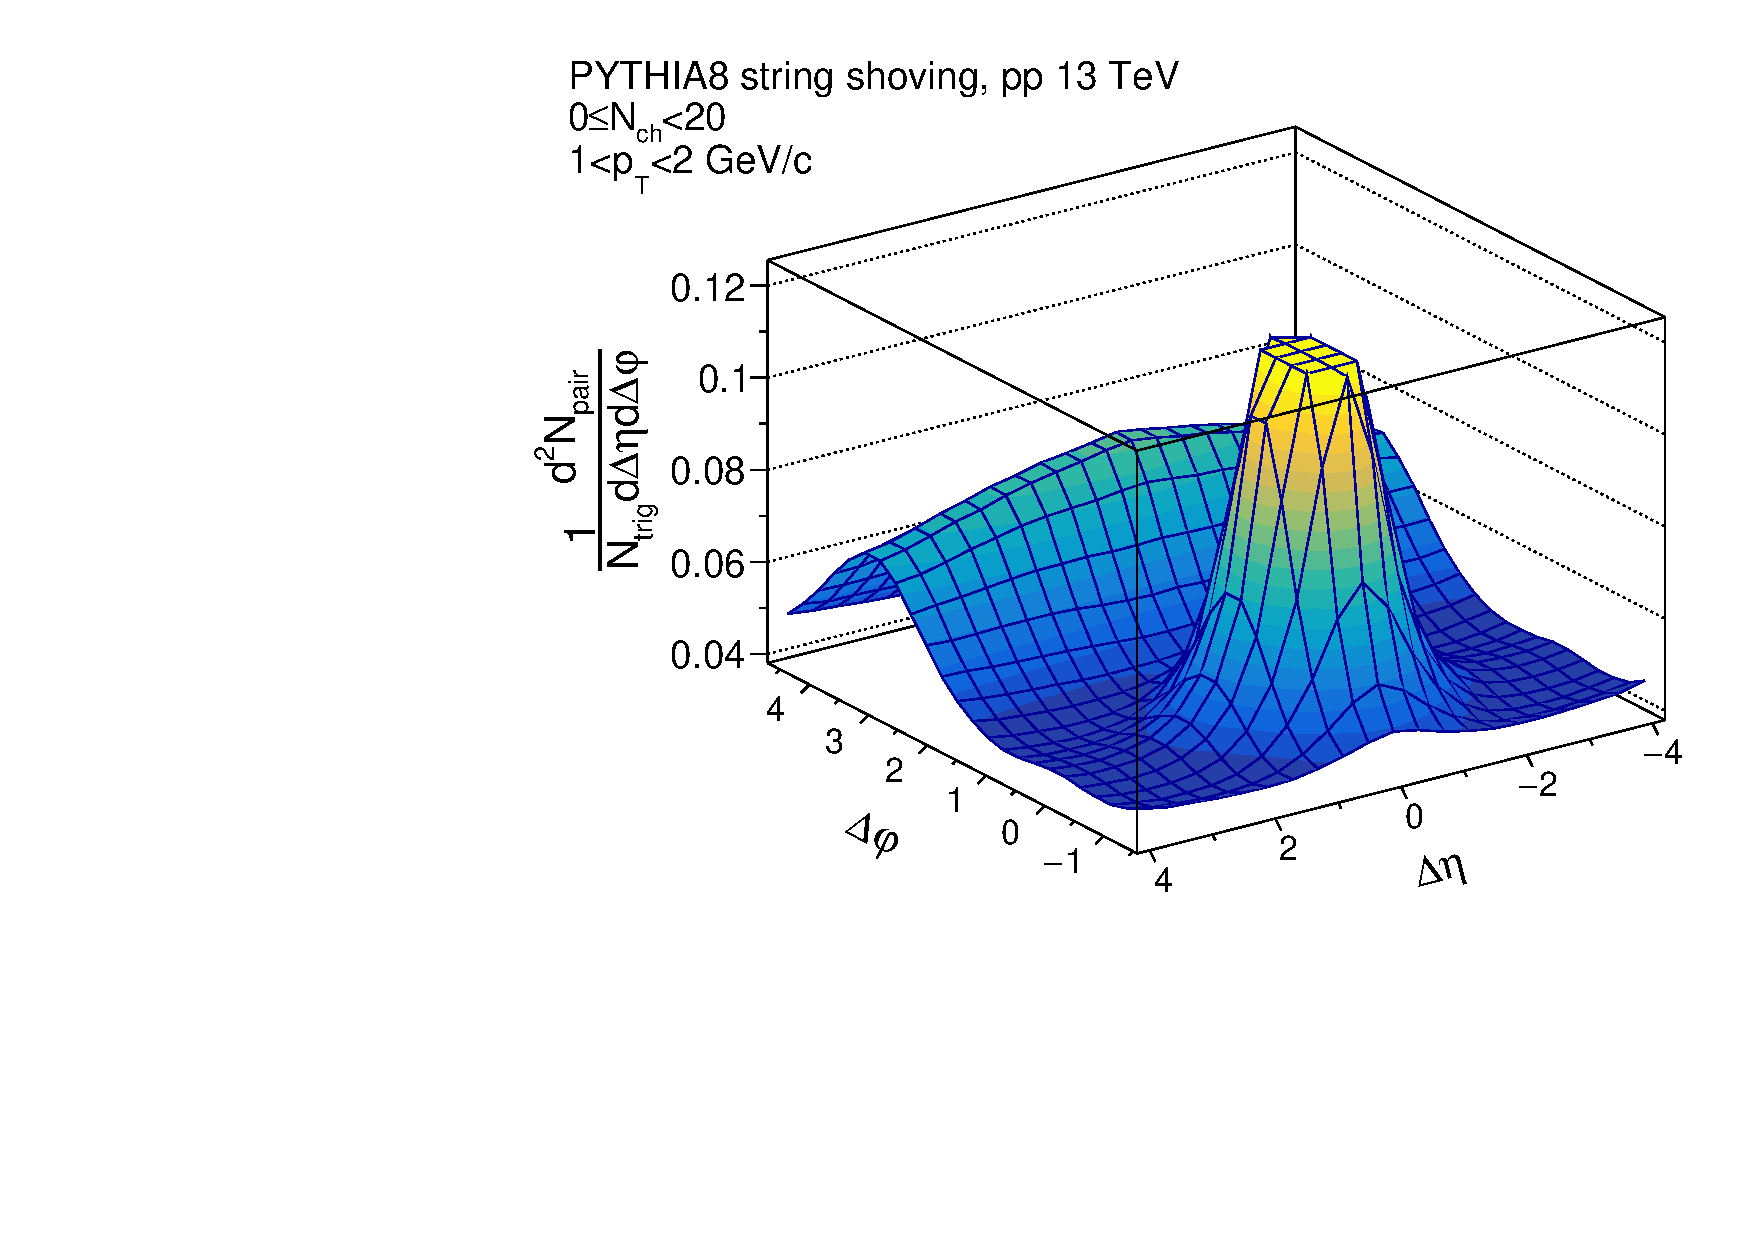
\includegraphics[width=0.49\textwidth]{figures/2D_shoving_lo_final.pdf}
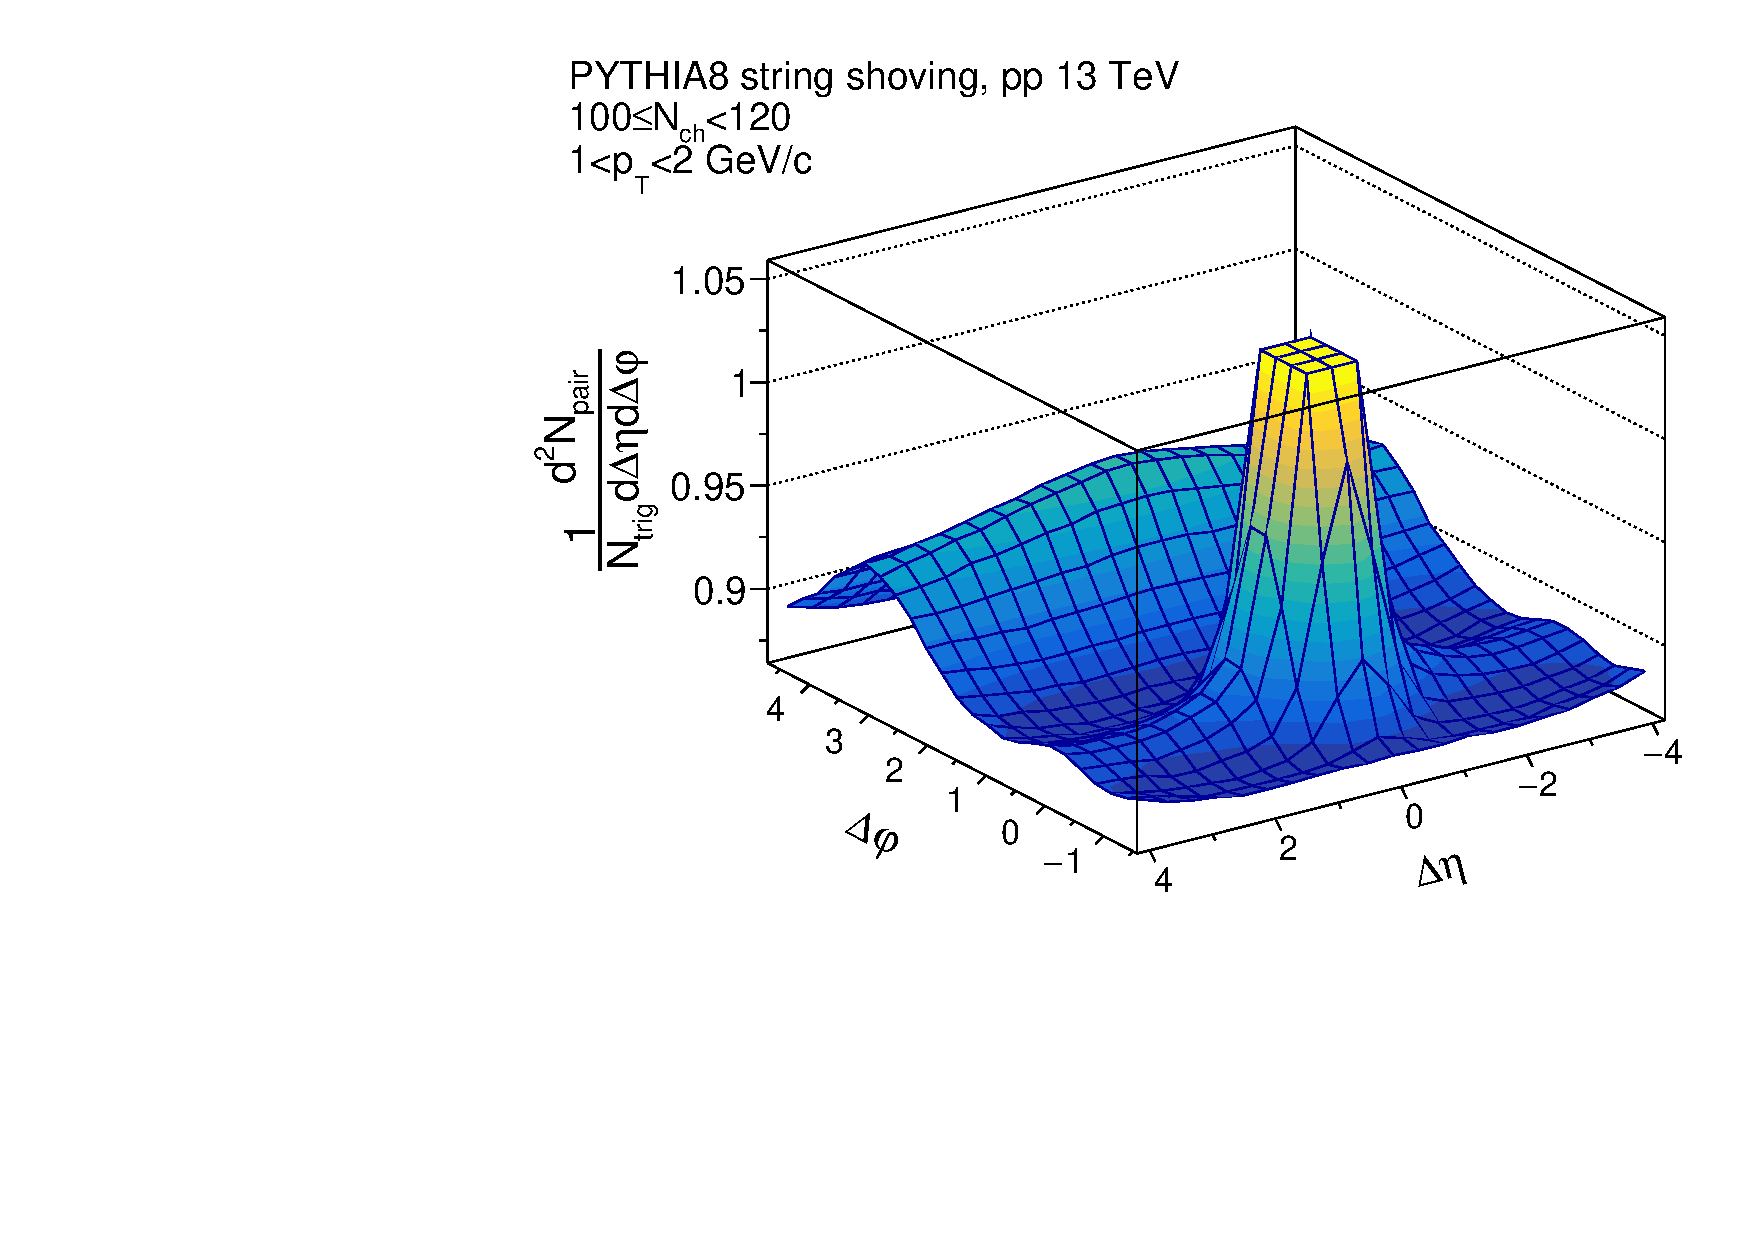
\includegraphics[width=0.49\textwidth]{figures/2D_shoving_hi_final.pdf}
\caption{Two-particle correlation functions for charged hadrons in $|\eta|<$~2.4 and 1~$<\pt<$~2~GeV/$c$ from low (left) and high (right) multiplicity \pythia \pp events at $\sqrt{s}=$~13~TeV with the string shoving model. \Nch is calculated with charged hadrons in $|\eta|<$~2.4 and $\pt>$~0.4~GeV/$c$.}
\label{fig:2d_shoving_final}
\end{figure}

\Cref{fig:2d_default_final,fig:2d_shoving_final,fig:2d_default_initial,fig:2d_shoving_initial} show two-particle \deta--\dphi correlation functions with charged hadrons for 1~$<\pt<$~2~GeV/$c$ in low (left) and high (right) multiplicity \pythia \pp events at $\sqrt{s}=$~13~TeV with different configurations. 
In \pythia events with the default configuration (Figure~\ref{fig:2d_default_final}), there is no long-range near-side correlation in two different multiplicity bins as expected. 
On the other hand, The correlation functions with the string shoving option shown in Figure~\ref{fig:2d_shoving_final} clearly exhibit a long-range near-side correlation called ``ridge''.
It is also worth mentioning that a ridge structure is observed even in low multiplicity events ($0\leq \Nch <20$) with the string shoving model, which is not seen in experimental results~\cite{Khachatryan:2015lva}.
For a closer look on correlations developed in the string shoving model, correlation functions with initial charged hadrons directly produced from partons are calculated as shown in \Cref{fig:2d_default_initial,fig:2d_shoving_initial}.
Like the correlation functions with final charged hadrons, a clear long-range near-side correlation is observed in events with the string shoving, whereas no such correlation is seen in events with the default configuration.
The ridge structure with initial charged hadrons is more prominent than one with final charged hadrons, and this implies that a smearing effect in decay processes decreases the correlation strength among particles. 

\begin{figure}[tbh]
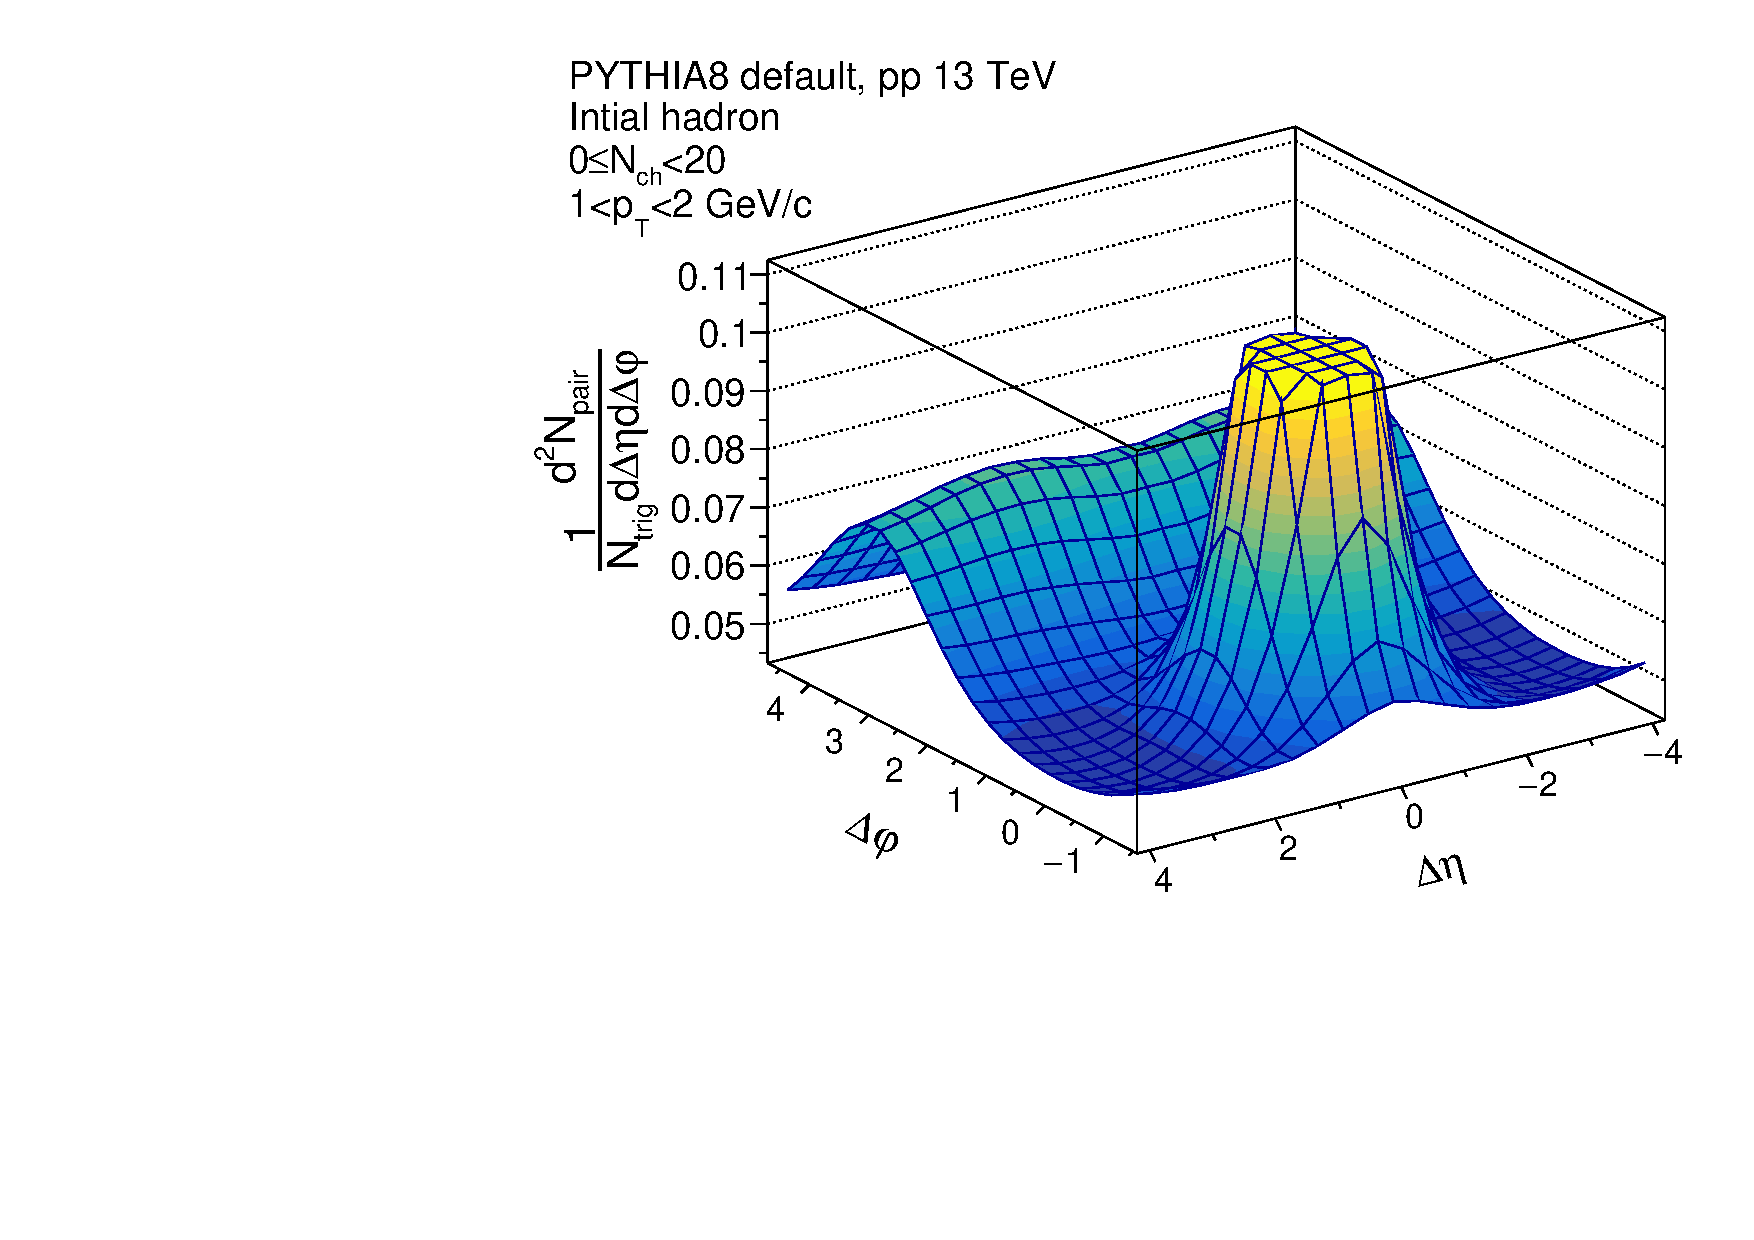
\includegraphics[width=0.49\textwidth]{figures/2D_default_lo_initial.pdf}
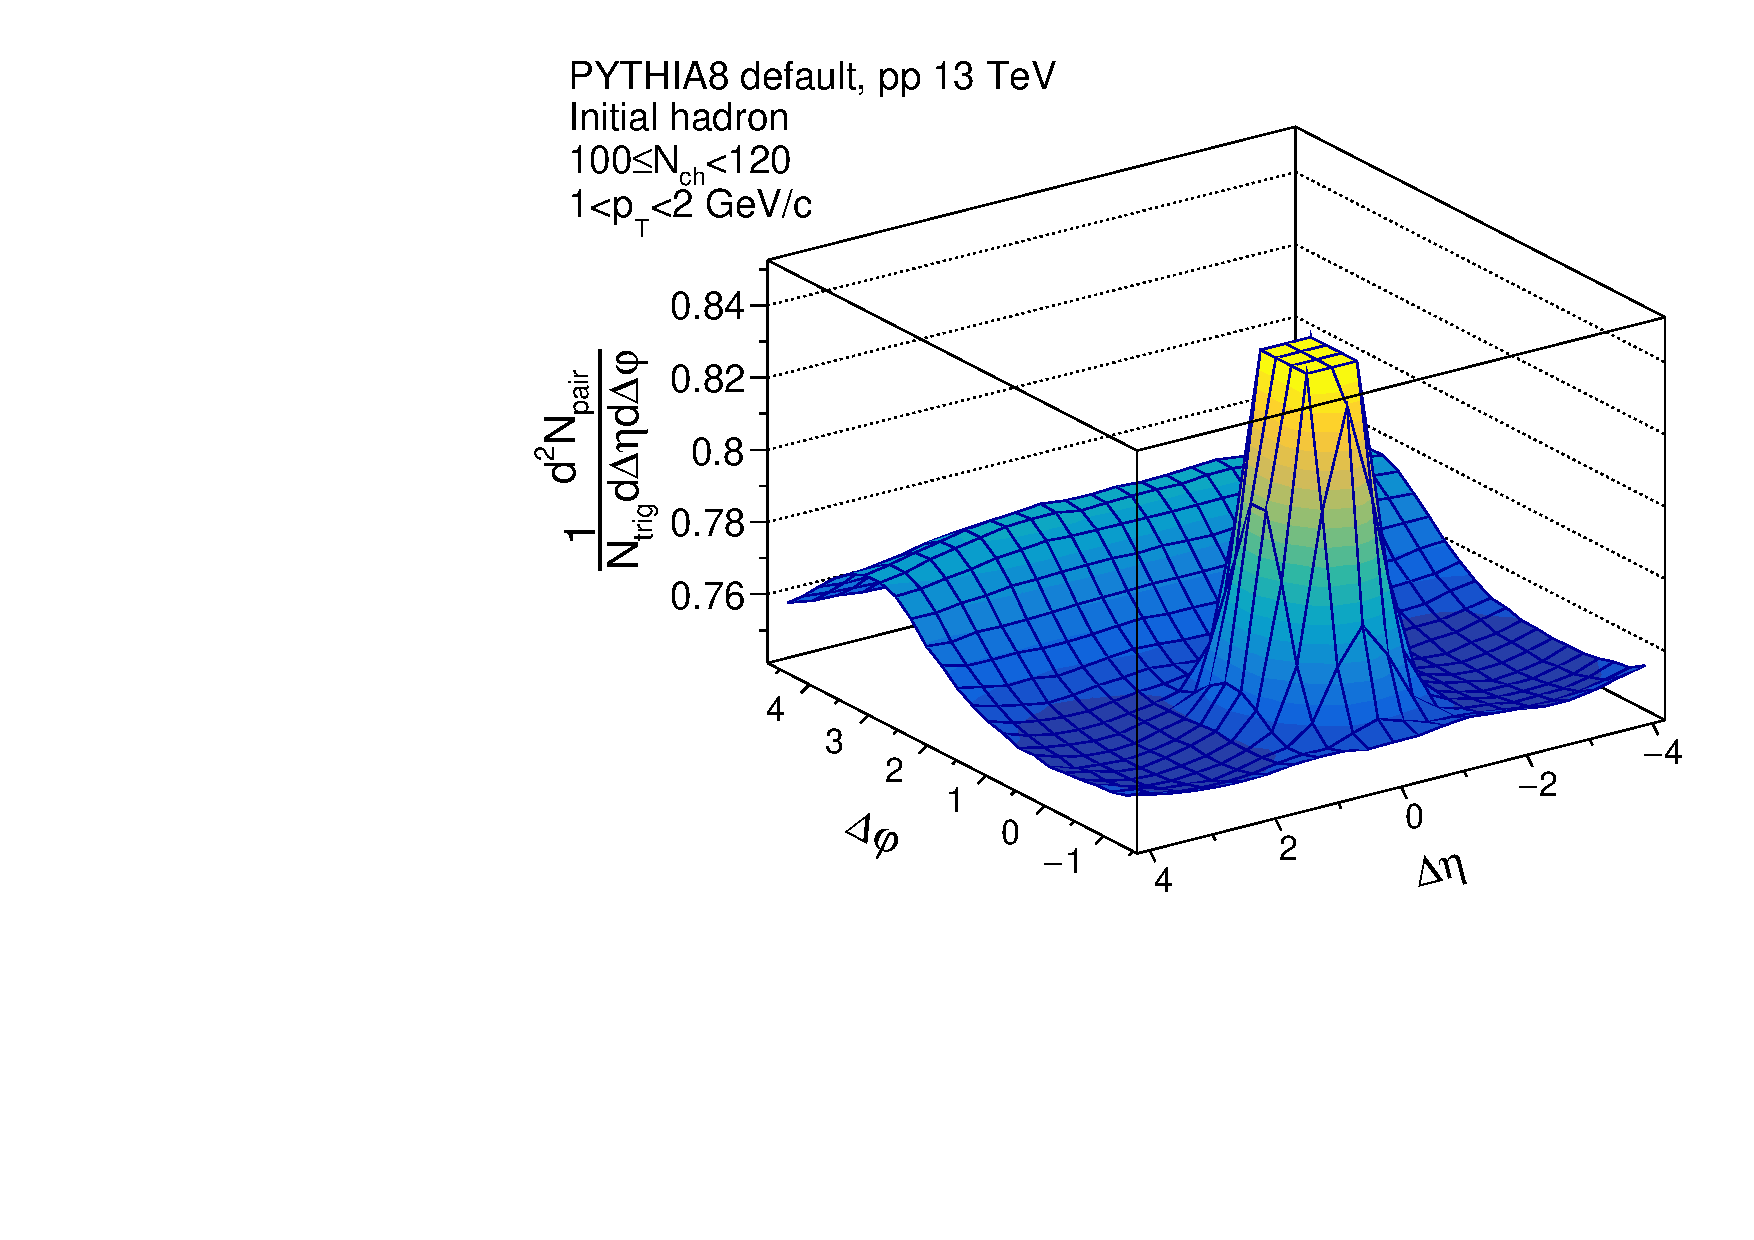
\includegraphics[width=0.49\textwidth]{figures/2D_default_hi_initial.pdf}
\caption{Two-particle correlation functions for charged hadrons in $|\eta|<$~2.4 and 1~$<\pt<$~2~GeV/$c$ from low (left) and high (right) multiplicity \pythia \pp events at $\sqrt{s}=$~13~TeV with the default configuration. Initial charged particles produced directly from partons are used for the correlations, and \Nch is calculated with final charged hadrons in $|\eta|<$~2.4 and $\pt>$~0.4~GeV/$c$.}
\label{fig:2d_default_initial}
\end{figure}

\begin{figure}[tbh]
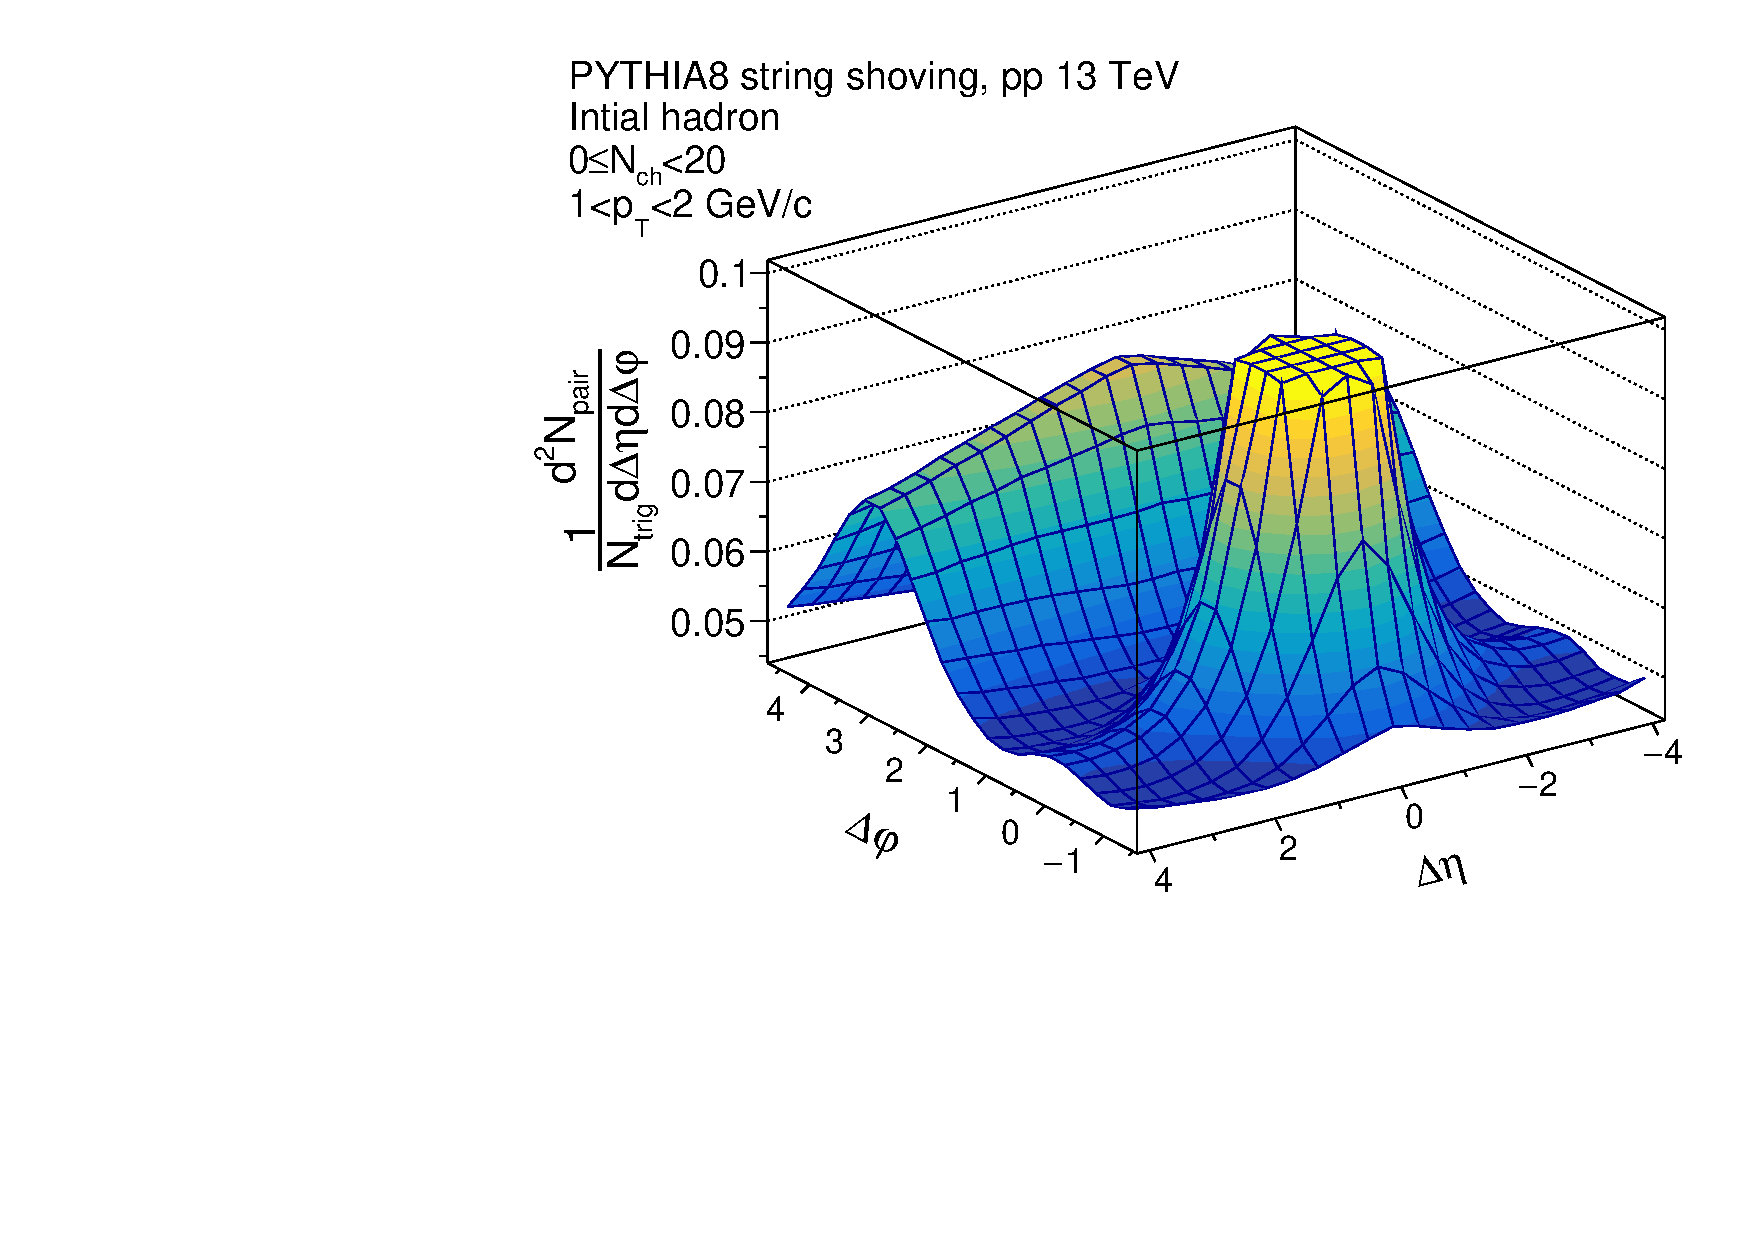
\includegraphics[width=0.49\textwidth]{figures/2D_shoving_lo_initial.pdf}
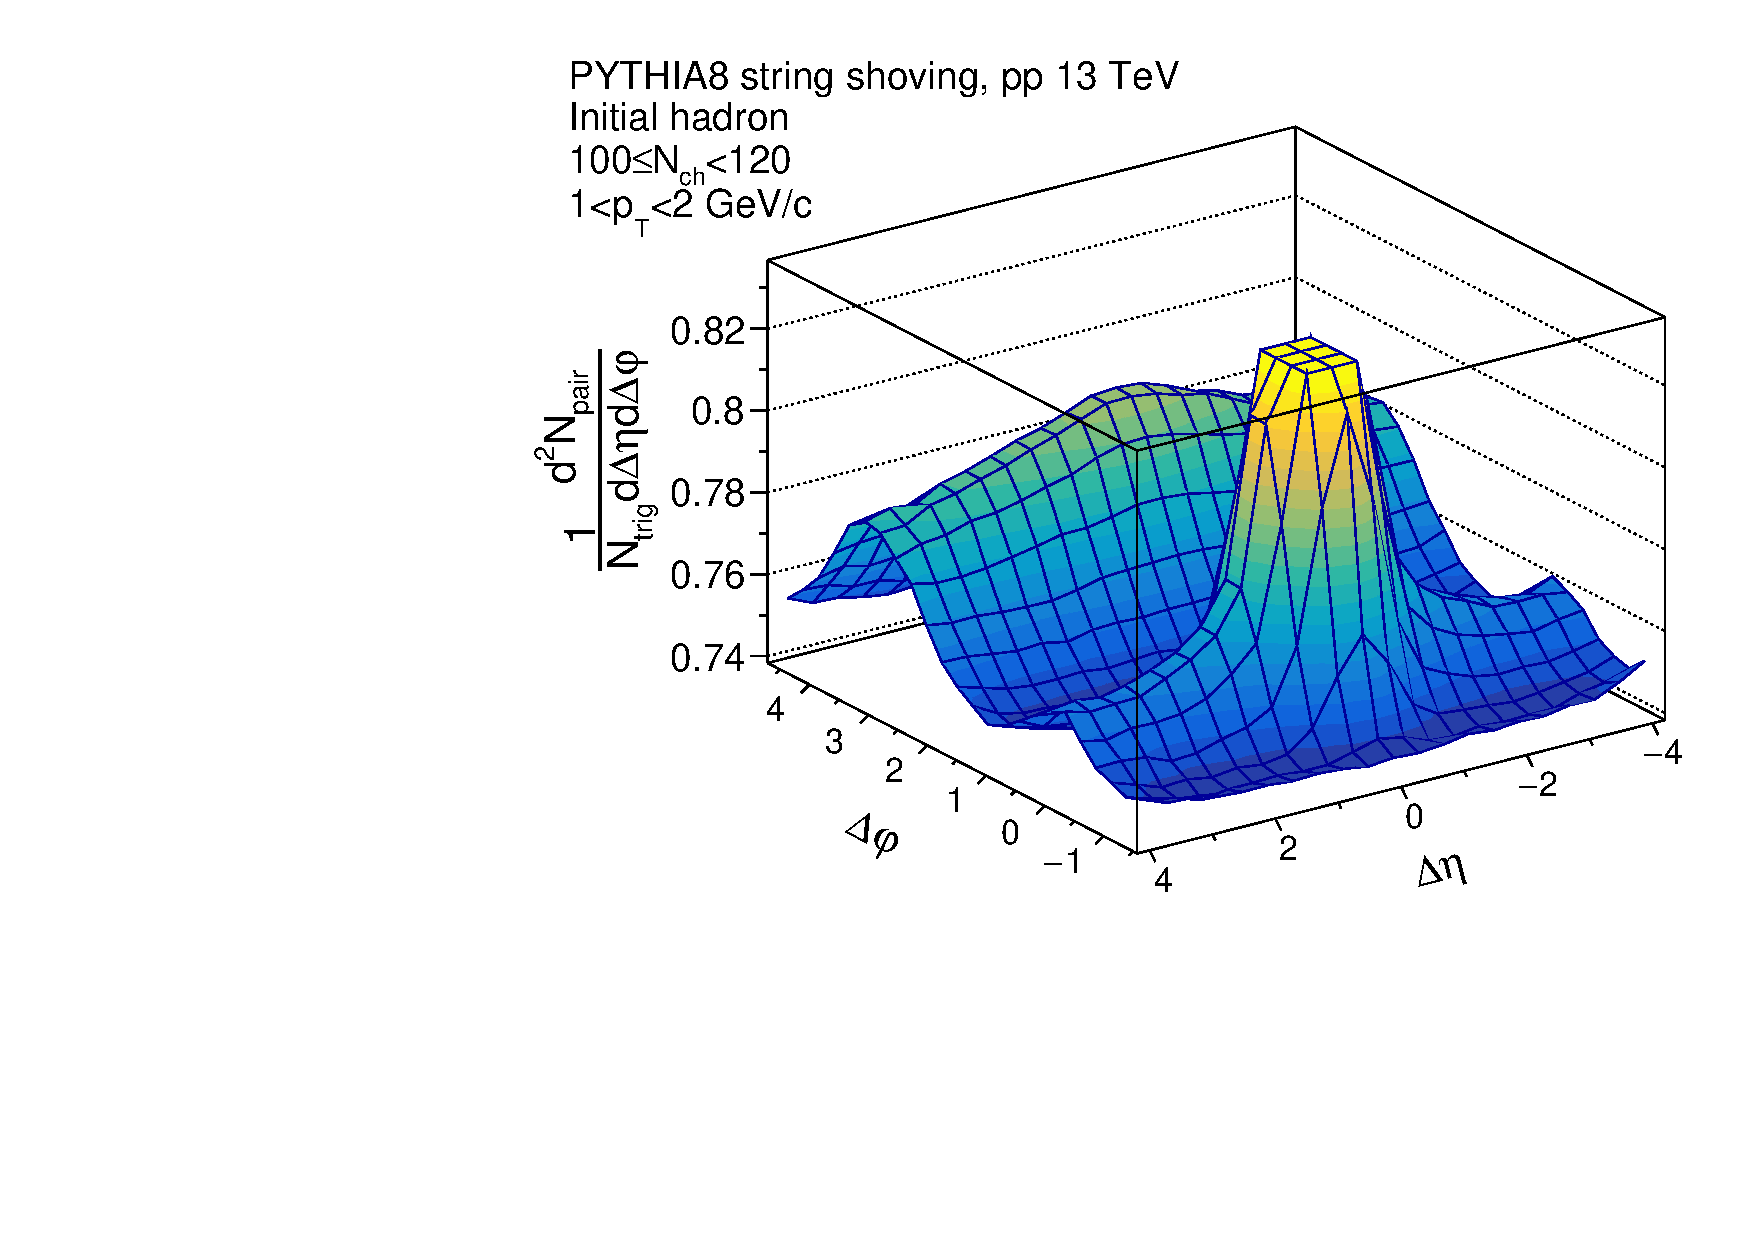
\includegraphics[width=0.49\textwidth]{figures/2D_shoving_hi_initial.pdf}
\caption{Two-particle correlation functions for charged hadrons in $|\eta|<$~2.4 and 1~$<\pt<$~2~GeV/$c$ from low (left) and high (right) multiplicity \pythia \pp events at $\sqrt{s}=$~13~TeV with the string shoving model. Initial charged particles produced directly from partons are used for the correlations, and \Nch is calculated with final charged hadrons in $|\eta|<$~2.4 and $\pt>$~0.4~GeV/$c$.}
\label{fig:2d_shoving_initial}
\end{figure}

One-dimensional \dphi correlation functions are constructed by averaging the two-dimensional correlation functions at a certain \deta range:
\begin{align}
\frac{1}{N_{\mathrm{trig}}} \frac{ \mathrm{d} N_{\mathrm{pair}} }{ \mathrm{d}\Delta\varphi } = \int \mathrm{d} \Delta \eta \frac{1}{\it{N}_{\mathrm{trig}}} \frac{ \mathrm{d}^{2} N_{\mathrm{pair}} }{ \mathrm{d}\Delta\eta d\Delta\varphi}.
\end{align}
For long-range correlations, the \deta range is determined as 2~$<|\deta|<$~4, where non-flow effects from di-jets and particle decay are expected to be not significant. 
The correlated part is estimated by implementing the Zero-Yield-At-Minimum (ZYAM) procedure~\cite{Ajitanand:2005jj}.
The minimum yield $(C_{\rm{ZYAM}})$ at the $\Delta\varphi$=$\Delta\varphi_{\rm{min}}$ for each \dphi correlation function is obtained by fitting the \dphi correlation function with a Fourier series up to the third term and is subtracted from the \dphi correlation function.
This procedure results in the \dphi correlation function at $\Delta\varphi_{\rm{min}}$ to be zero.

Figure~\ref{fig:dphi} shows one-dimensional \dphi correlation functions at long-range (2~$<|\deta|<$~4) after applying the ZYAM procedure for different \pt ranges in low (upper) and high (lower) multiplicity events.
\pythia events with the default configuration show no near-side structure in different \pt and multiplicity ranges. 
\pythia events with the string shoving option, on the other hand, clearly show near-side peaks.
The CMS results~\cite{Khachatryan:2015lva} are compared with the correlation functions from \pythia events, and the multiplicity ranges for \pythia events are selected $\sim15\%$ higher than the multiplicity ranges for CMS results to consider a track reconstruction efficiency.
The string shoving model overestimates near-side correlation for 1~$<\pt<$~2~GeV/$c$ in low multiplicity events.
In the high multiplicity range, the correlation function of final charged hadrons for 1~$<\pt<$~2~GeV/$c$ in \pythia events with the string shoving nicely agrees with the CMS result.
However, the model underestimates the near-side correlation for higher \pt ranges. 


\begin{figure}[!h]
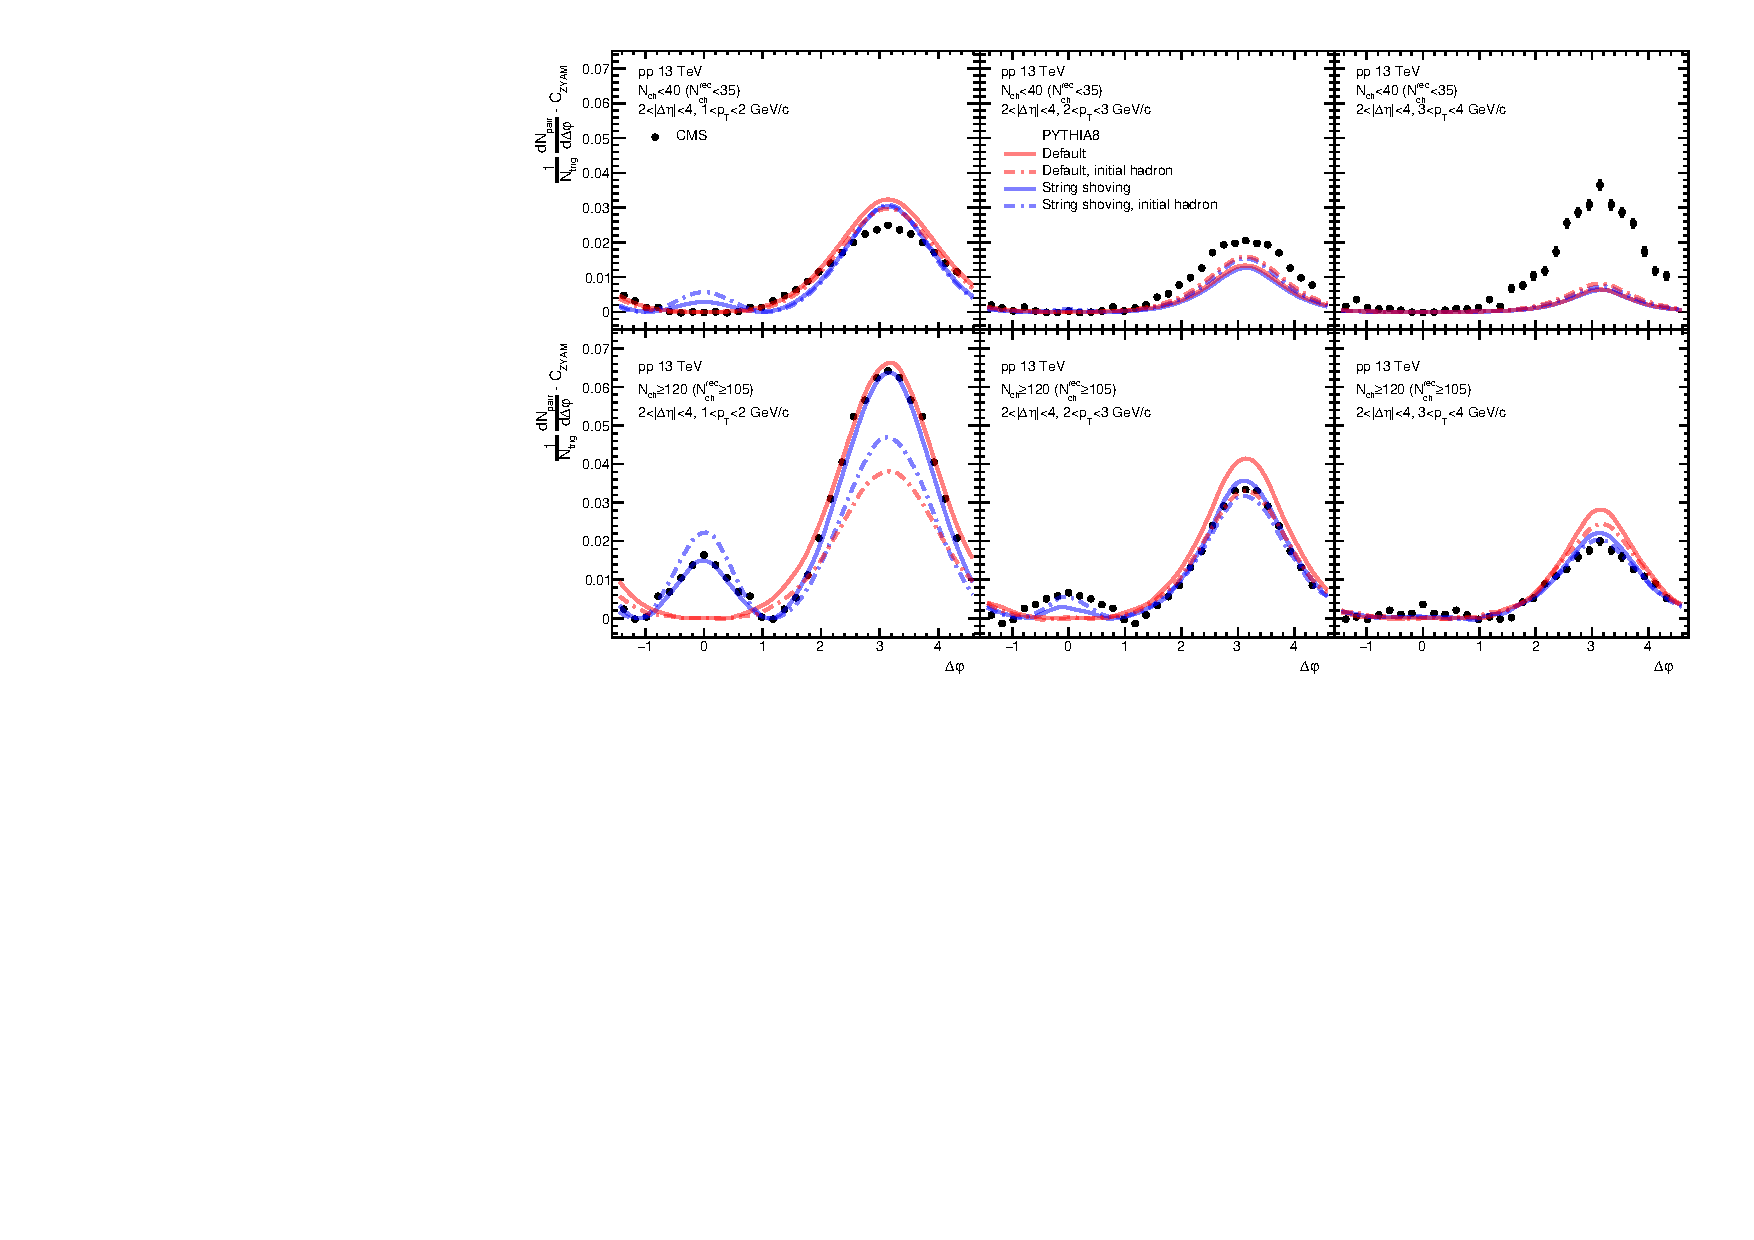
\includegraphics[width=1.0\textwidth]{figures/dphi_all2.pdf}
\caption{One-dimensional long-range (2~$<|\Delta\eta|<$~4) $\Delta\varphi$ correlations in low and high multiplicity events for different \pt bins. The CMS results (closed circle)~\cite{Khachatryan:2015lva} are compared with correlation functions using initial (dashed) and final (solid) charged hadrons from \pythia events with (red) and without (blue) the string shoving.}
\label{fig:dphi}
\end{figure}
